\chapter{Gravitation and astrophysics}\label{ch:Let-there-be-gravity}

\section{What goes up\ldots}

\subsection{Newton}

Gravity is one of the fundamental forces of nature, familiar as the force that keeps the Earth in orbit about the Sun and makes falling off a log so easy. \citet[book 3]{Newton1999} was the first to realise that gravity is universal and the same force explains both apples dropping from trees and the motion of celestial bodies. In the \textit{Principia}, first published in 1687, he outlined a gravitational force that scaled as the inverse of the square of the distance between the centres of mass and was proportional to the product of the masses of the bodies. In modern notation, the force is
\begin{equation}
F = \dfrac{G m_1 m_2}{r^2},
\end{equation}
for distance $r$, masses $m_1$ and $m_2$, and gravitational constant $G$. This theory has been hugely successful. Not only is it still taught in schools today, but it is also used for astronomical research. Newton's law of universal gravitation has proved accurate in describing orbital motions. However, there are observations that do not fit its predictions.

In the early nineteenth century, the motion of Uranus was found to deviate from its expected trajectory. Rather than seeking to modify the theory, \citet[\textit{troisi{\`e}me partie}]{LeVerrier1846} and \citet[papers 1, 2]{Adams1896} calculated the properties of a perturbing object that could explain the motion. They predicted the existence of an unseen mass, a new planet; this was subsequently observed within a degree of Le Verrier's hypothesised position \citep[\textit{cinqui{\`e}me partie}]{LeVerrier1846} and became known as Neptune.

Newtonian gravity survived the trial of Uranus' orbit, but it could not explain the perihelion precession of Mercury. \citet[\textit{chapitre XV}, \textit{section quatri{\`e}me}]{LeVerrier1859} first noticed the anomaly. A new inner planet was suggested, but this time it could not be found. What was needed was a modified theory of gravitation: the Newtonian theory is insufficient in the stronger gravity close to the Sun \citep[document 24]{Einstein1997}.

\subsection{Einstein}

The new extended theory was General Relativity (GR), developed by Einstein in the 1910s \citep{Einstein1997}. This describes gravity as the effect of the curvature of spacetime, which is now a dynamical entity. Particles naturally travel along geodesics of spacetime, which may appear curved; the curvature of spacetime itself is sourced from the energy-momentum it contains: matter tells spacetime how to curve, and spacetime tells matter how to move \citep[section 1.1]{Misner1973}. This is encapsulated within the Einstein field equations \citep[documents 22, 25]{Einstein1997}
\begin{equation}
R_{\mu\nu} - \recip{2}R g_{\mu\nu} = \dfrac{8\pi G}{c^4}T_{\mu\nu},
\end{equation}
where $g_{\mu\nu}$ is the metric, $R_{\mu\nu}$ and $R = g^{\mu\nu}R_{\mu\nu}$ are the Ricci tensor and scalar (\citealt[section 8.7]{Misner1973}; \citealt[section 3.2]{Wald1984}), $c$ is the speed of light, and $T_{\mu\nu}$ is the energy-momentum tensor.\footnote{Our definition for the Ricci tensor is given in \nameref{conventions}.} GR reduces to its Newtonian counter-part in the weak-field limit, or conversely, it extends Newtonian gravity to stronger gravitational fields.

Since its inception, GR has successfully passed every observational test \citep{Will1993, Will2006}. However, astronomers have not been idle, and the twentieth century has yielded further surprises.

Observations of the velocity dispersions of galaxies in clusters are higher than those calculated from the quantity of luminous matter \citep[e.g.,][]{Zwicky1937}. Similarly, measurements of the rotation curves of galaxies do not match the expected profile \citep{Babcock1939}. Gravitational lensing of galaxy clusters confirms that their gravity is dominated by an unseen component \citep{Bergmann1990,Clowe2006}. This has been interpreted as motivation for introducing dark matter, a new component of the Universe that gravitates but does not emit or absorb electromagnetic (EM) radiation. Dark matter has become central to our understanding of cosmology \citep[e.g.,][]{Springel2006a}; it is needed to explain structure formation: without it we could not form galaxies from the small over-densities inferred from the homogeneity of the cosmic microwave background (CMB; \citealt{White1978,Liddle1993}). Although we know the properties required of dark matter and we can estimate the required energy density, we do not have a definite candidate for a dark matter particle \citep{Bertone2005}; its true nature remains a mystery.

Observations of type IA supernovae have revealed that the Universe is not only expanding, but is accelerating \citep{Riess1998,Perlmutter1999}. This acceleration has been attributed to the influence of dark energy \citep{Perlmutter1999a,Peebles2003}. The nature of dark energy is even more mysterious than that of dark matter. The simplest explanation is to introduce a cosmological constant $\Lambda$; this modifies the Einstein field equations to become \citep[document 43]{Einstein1997}
\begin{equation}
R_{\mu\nu} - \recip{2}R g_{\mu\nu} - \Lambda g_{\mu\nu} = \dfrac{8\pi G}{c^4}T_{\mu\nu}.
\end{equation}
This model has been highly successful in explaining the evolution of the Universe, but we still do not know if a cosmological constant is the true explanation and if so, why it has its particular value \citep{Carroll2001}. A possible alternative is the presence of a slowly evolving scalar field \citep{Copeland2006}.

\subsection{This work}

Despite the long history of its study, we still do not know everything about gravity. There are still discoveries to be made. Gravity is the weakest of the fundamental forces and so is difficult to study in the laboratory. Yet it dominates on astronomical scales; understanding gravity is crucial to understanding the cosmos. We have learnt much about the workings of the Universe through improving our understanding of gravity, and the motivation for developing new theories of gravitation has often come from astronomical observations. Gravitation and astrophysics are intimately linked.

This thesis is divided into two strands. The first (\partref{astro}) is concerned with what we could learn about astrophysical systems from gravitational probes; the second (\partref{grav}) is concerned with what we can learn about gravity from astronomical observations. We shall consider strong-field tests and, in particular, gravitational waves (GWs). The former part concentrates on what we could hope to learn about massive black holes (MBHs) and their surrounding stellar environment from extreme-mass-ratio bursts (EMRBs); the latter looks at both modifications to gravity in metric $f(R)$ theory and the effects of transient resonances in GR.

To introduce these topics, we review in \secref{strong-field} possible means of probing gravitational phenomena. GWs are the perfect means of investigating the strong-field regime, which has yet to be fully mapped. The strongest gravitational fields are found in the vicinity of compact objects (COs), such as black holes (BHs). We describe these objects in \secref{COs}. MBHs are a particularly interesting class of COs, since they may be linked to galaxy evolution and trace out cosmological structure formation. This is why we shall study what EMRBs could teach us about them. To successfully interpret GW observations, we must have a solid understanding of gravity. There are many alternatives to GR, which we discuss in \secref{alternative}. We shall study $f(R)$-gravity, in an effort to explore the possible ways that gravity could be modified. To make either precision measurements of astrophysical objects or exacting tests of GR it is necessary to have accurate predictions for waveforms in GR. We discuss the general relativistic two-body problem in \secref{two-body}. We shall go on to investigate the effects of transient resonances, which could introduce a small error in existing modelling techniques. Since GW astronomy is a new field, there is great potential for unexpected revelations.

\section{Strong-field tests and gravitational waves}\label{sec:strong-field}

The deviations from Newtonian theory were first noted in the gravitational field close to the Sun, the strongest accessible in the Solar System. GR has now been tested in stronger fields \citep{Will2006}, but there are still more extreme systems to be explored. It is here that we expect any deviations to manifest. We know that our understanding of GR in the strongest fields is, at the least, incomplete: BHs feature singularities at their centres, where the theory breaks down (\citealt[section 34.6]{Misner1973}; \citealt[chapter 9]{Wald1984}). Even if we do not find any deviations from GR, it is still worthwhile to check its validity, if only as a matter of scientific principle.

\subsection{Field strength and existing tests}\label{sec:exist-tests}

In order to parameterize the strength of gravity, \citet{Psaltis2008a} introduces two characteristic quantities: the dimensionless potential or compactness \citep{Yunes2013}
\begin{equation}
\varepsilon = \dfrac{GM}{rc^2} = \dfrac{r\sub{g}}{r},
\end{equation}
and the dimensionful curvature
\begin{equation}
\xi = \dfrac{GM}{r^3c^2} = \dfrac{r\sub{g}}{r^3},
\end{equation}
where $M$ is the gravitating mass, $r$ a characteristic distance and $r\sub{g}$ is the gravitational radius. These are larger for stronger fields. The potential ranges from $\varepsilon \simeq 0$ in weak fields to $\varepsilon \sim \order{1}$ near the surface of a neutron star (NS) or a BH event horizon. It is useful in defining post-Newtonian (PN) expansions. The curvature $\xi$ approximates the form of the Riemann tensor, which is fundamental to GR. It is necessary to pick a particular reference scale to define when the curvature becomes large; however, it is a useful gauge of the strength of a gravitational field in a geometric theory because it is the lowest order measure that cannot be eliminated by a coordinate transformation \citep[chapter 7]{Hobson2006}.

Using these two parameters, we can map out the possible tests of GR. \Figref{Psaltis} shows a selection of current astrophysical tests.
\begin{figure}
  \centering
  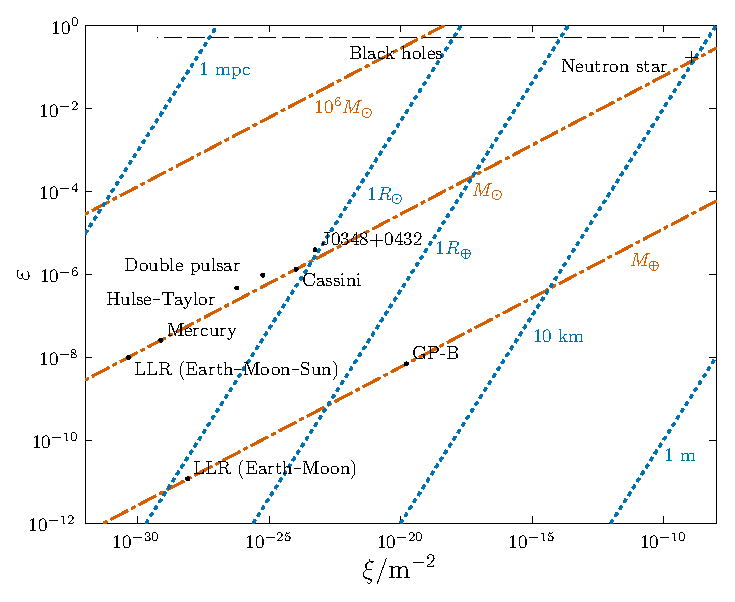
\includegraphics[width=0.6\textwidth]{./images/Fig_Psaltis_plot}
    \caption{Astrophysical tests of GR parameterized by the compactness and curvature scales they probe, adapted from \citet{Psaltis2008a}. The dashed line indicates the Schwarzschild radius $r\sub{S} = 2 r\sub{g}$ for BHs of mass $5$--$10^{11} M_\odot$ and the cross indicates the surface of an NS. The dotted line and the dot--dashed line indicate the scales accessible at a given radius and mass respectively.}  
    \label{fig:Psaltis} 
\end{figure}
Included are:
\begin{itemize}
\item The classic perihelion precession of Mercury (\citealt[section 10.2]{Hobson2006}; \citealt[section 7.3]{Will1993}; \citealt{Pitjeva2013});
\item Doppler tracking of the Cassini--Huygens spacecraft \citep{Bertotti2003} which measures the time delay of light travelling past the Sun \citep[section 7.2]{Will1993};
\item Lunar laser ranging (LLR; \citealt{Bender1973,Williams2012}) which provides precise measurements of the orbits of the Earth--Moon and Earth--Moon--Sun systems \citep[section 8.1]{Will1993};
\item Gravity Probe B (GP-B; \citealt{Everitt2009,Everitt2011}) which produced measurements of the geodetic drift and frame-dragging \citep[section 9.1]{Will1993};
\item A selection of binary pulsars \citep{Taylor1993,Stairs2003}, specifically the Hulse--Taylor binary (PSR B1913$+$16; \citealt{Hulse1975,Weisberg2010}), which was the first discovered and the first system to show the influence of GWs; PSR J0348$+$0432 \citep{Antoniadis2013} which includes a $2 M_\odot$ pulsar, and the double pulsar system (PSR J0737$-$3039; \citealt{Breton2008,Kramer2008}). There are many other pulsar systems, for example PSR B1534+12, a double-NS system closer than the Hulse--Taylor binary \citep{Stairs2002}, and PSR J1738+0333, which has an optically observable WD companion \citep{Antoniadis2012} and can be used to place strong constraints on scalar--tensor theories of gravity \citep{Freire2012}.
\end{itemize}
For comparison, we have also plotted the parameters for the surface of an NS and the Schwarzschild radius of BHs of various masses. BHs range in mass from a few solar masses \citep{Ozel2010} to several billion solar masses \citep{Hlavacek-Larrondo2012}. To probe the strongest fields, we need a way of probing the spacetime of COs like NSs and BHs.

In addition to the astrophysical tests of gravity, it is possible to make precision tests in the laboratory \citep{Kapner2007a,Adelberger2009,Wagner2012}. Whilst these are limited to using small masses, they do allow careful control of the system that is not possible in astronomy. Neither the astrophysical nor the laboratory tests performed so far show any discrepancy from the predictions of GR \citep{Will2006}. 

\subsection{Gravitational radiation}

One particularly promising method of exploring strong-field regions would be to observe GWs. These are predicted in any relativistic theory of gravity, where changes in the gravitational field must propagate at finite speed \citep{Schutz1984}. Within GR they are tiny ripples in the spacetime metric (\citealt[section 35.1]{Misner1973}; \citealt[section 107]{Landau1975}). They are generated by systems with a time-varying mass quadrupole; significant gravitational radiation originates from regions where spacetime is highly dynamic and the objects are extremely relativistic. This is precisely the strong-field domain we are interested in investigating.

Some intuition about GWs can be obtained from the more familiar EM waves (\citealt[sections 46--48, 66--67]{Landau1975}; \citealt[sections 7.1, 9.1--9.3]{Jackson1999}). These are oscillations of the electric and magnetic fields produced by accelerating charges whilst GWs are oscillations of the spacetime metric produced by accelerating masses. EM waves may be sourced by a time-varying charge dipole; as a consequence of conservation of momentum there is no time-varying mass dipole, so GWs are sourced by the mass quadrupole (\citealt[section 18.5]{Hobson2006}; \citealt[section 15.4]{Rindler2006}). Both waves propagate at the speed of light and have two (transverse) polarizations: for GWs these represent two orthogonal patterns of stretching and squeezing as shown in \figref{plus-cross} (\citealt[section 34]{Dirac1996}; \citealt[section 18.4]{Hobson2006})
\begin{figure}
  \centering
  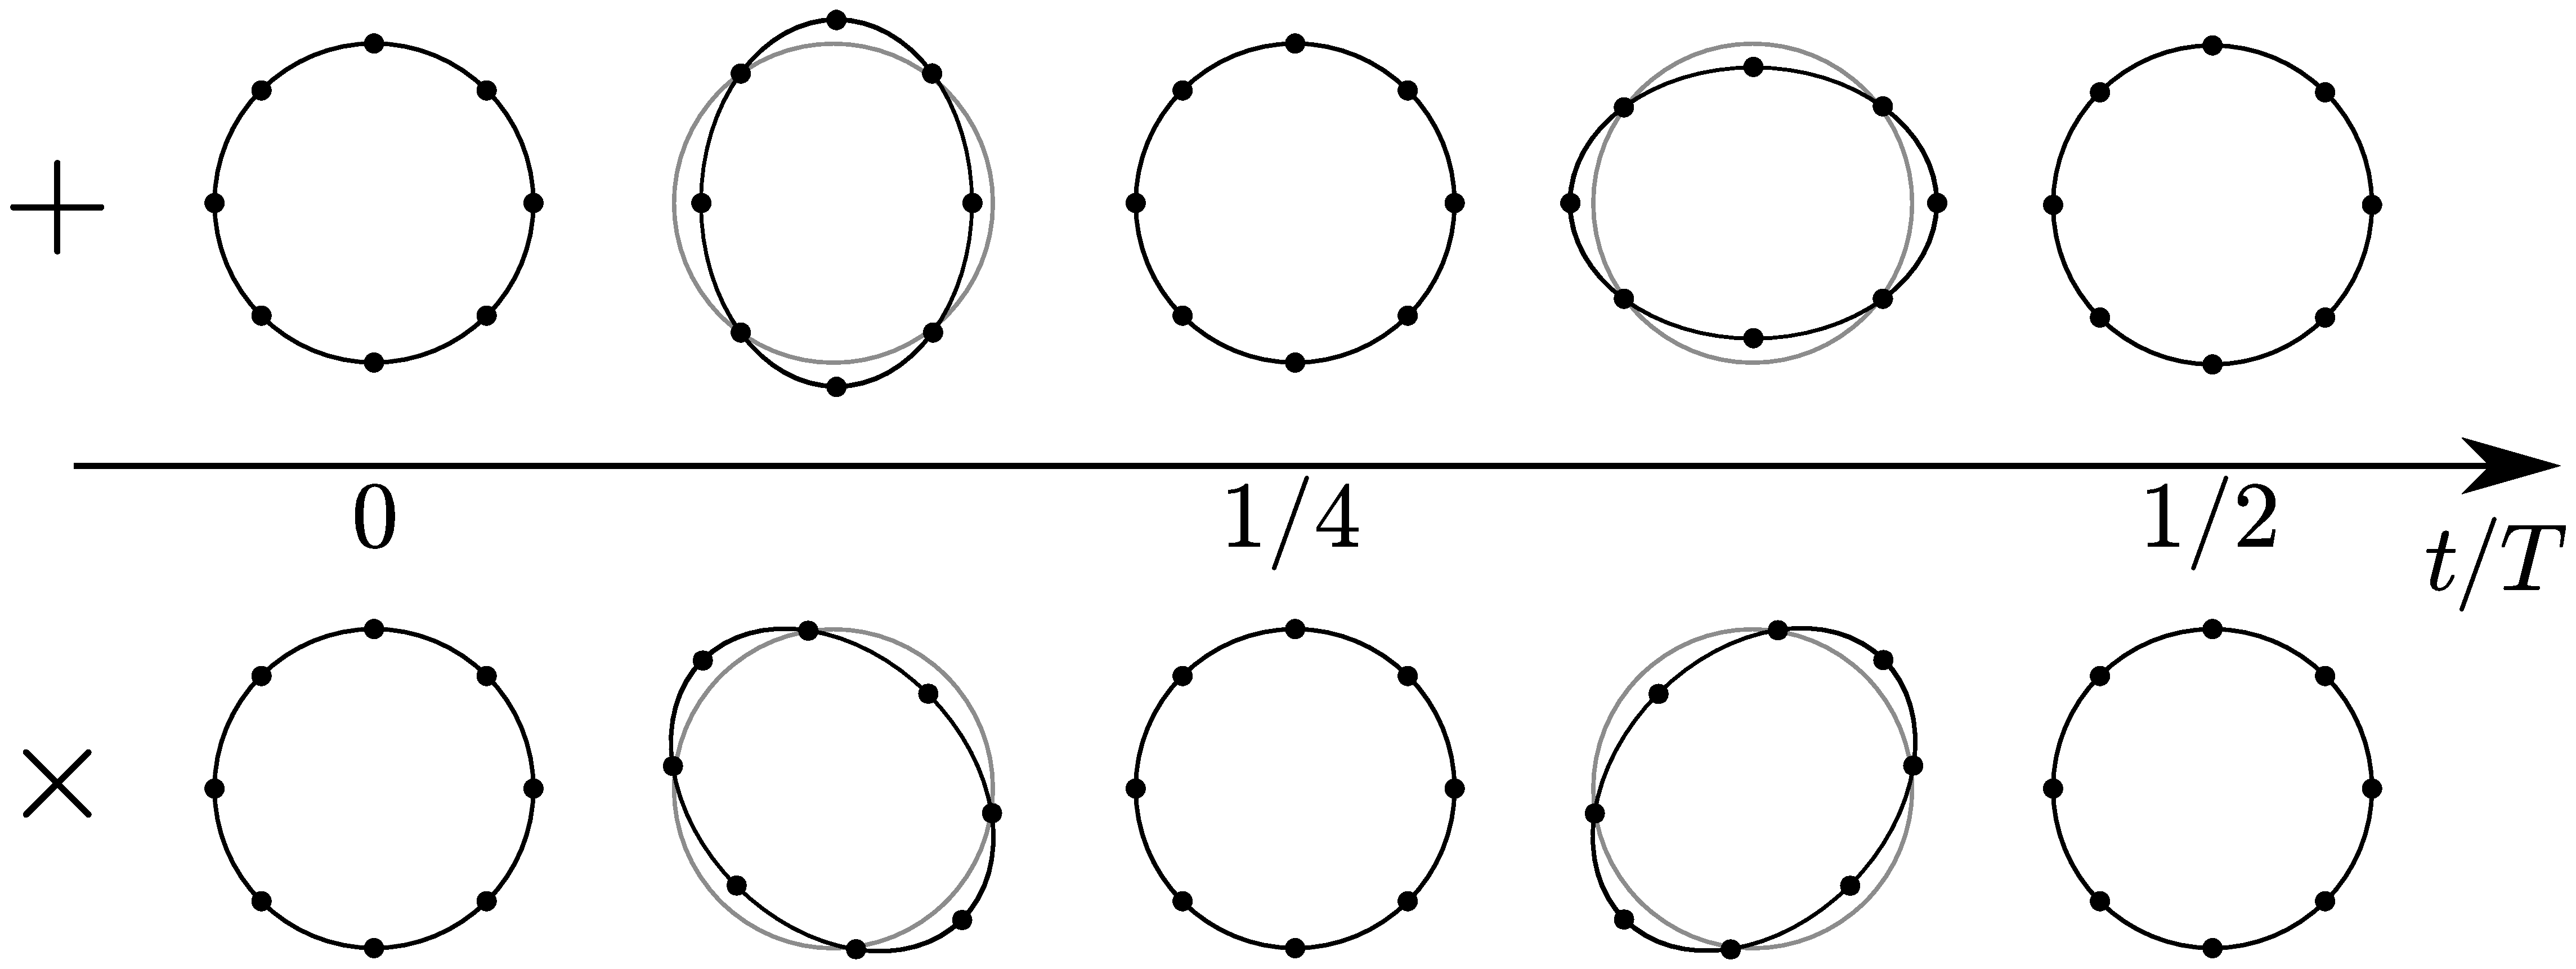
\includegraphics[width=0.7\textwidth]{./images/Polarization}
    \caption{The effect of the two GW polarizations (plus $+$ and cross $\times$) on a ring of free particles as a function of time. The propagation direction is perpendicular to the ring. The wave period is $T$.}   
    \label{fig:plus-cross} 
\end{figure}

Visible light has been used by astronomers for millennia. In the twentieth century, the useful spectrum was extended through infrared to radio, and from ultraviolet to X-rays and gamma rays \citep[chapter 7]{Longair2006}. In the twenty-first century, we hope to move from EM to gravitational radiation. GWs encode valuable information about their sources, information that is inaccessible by other means.

Just like EM waves, GWs come in a range of frequencies. The frequency is set by the scale of the source system: typically, more massive objects have longer associated time-scales, as these can be no shorter than the light-crossing time $t\sub{g} = r\sub{g}/c$, and so produce lower frequency radiation. \Figref{spectrum} shows the GW spectrum with illustrative detectors and sources.
\begin{figure}
  \centering
  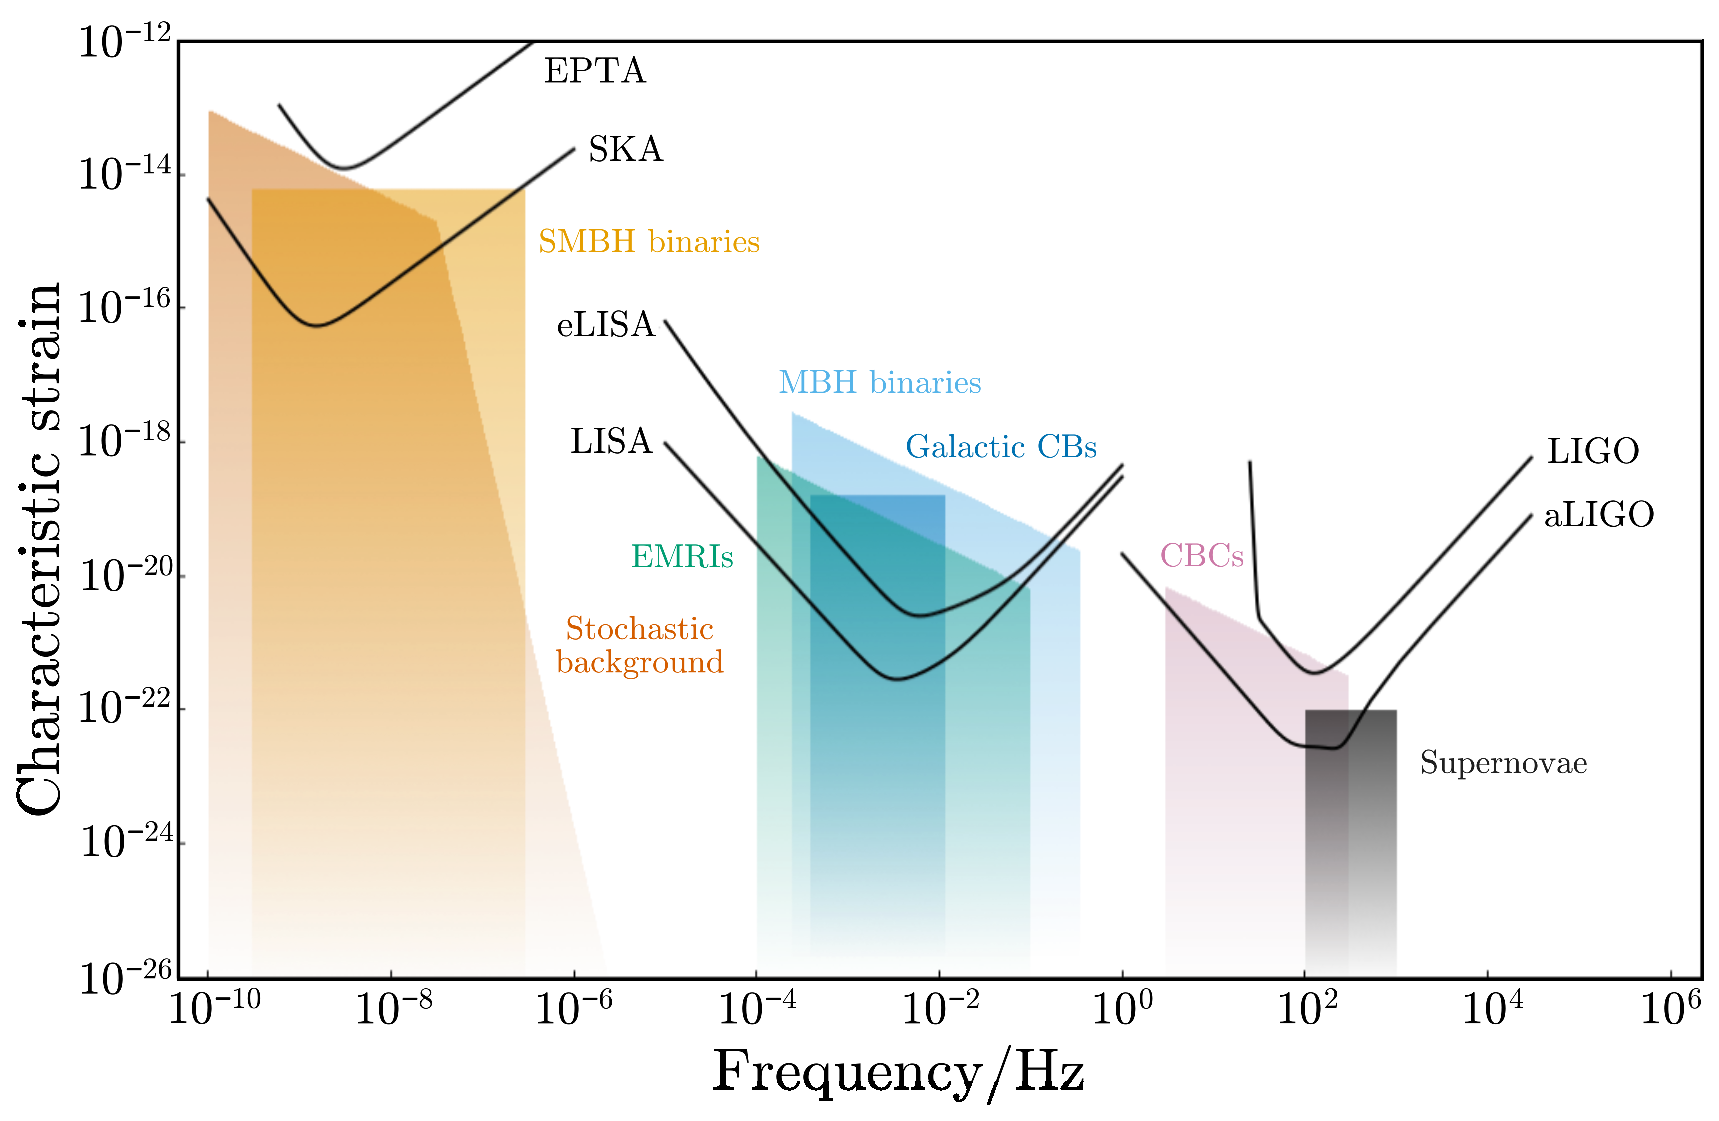
\includegraphics[width=0.7\textwidth]{./images/GW_spectrum}
    \caption{Cartoon spectrum of GWs. Sources (see \secref{GW-sources}) are indicated by their characteristic amplitude as measured on Earth, detectors (see \secref{GW-det}) are characterised by their sensitivity curves. Adapted from \url{http://www.ast.cam.ac.uk/~rhc26/sources/}.}   
    \label{fig:spectrum} 
\end{figure}
Detectors are sensitive to specific frequency bands, the range of which is set by their size. The spectrum may be divided into: the extremely low frequency (ELF; not shown in the figure) regime, $\sim10^{-18}$--$10^{-15}\units{Hz}$, which may be indirectly detected through observations of the polarization of the CMB \citep[e.g.,][]{Hu1997,Kamionkowski1997}; the very low frequency (VLF) regime, $\sim10^{-9}$--$10^{-6}\units{Hz}$, which is accessible to pulsar timing arrays (PTAs); the low frequency (LF) regime, $\sim10^{-6}$--$1\units{Hz}$, which could be measured by space-borne detectors, and the high frequency (HF) regime, $\sim1$--$10^4\units{Hz}$, which is the target range for ground-based detectors. Individual detectors are discussed in \secref{GW-det} and some example sources are introduced in \secref{GW-sources}.

While GWs are an exciting source of information, it will be beneficial to compare with results from other techniques, to maximise the data available for inferences, and to check models. For example, very long baseline interferometry (VLBI) may be used to image the vicinity of a BH's horizon \citep{Doeleman2008,Johannsen2012a}, or X-ray observations could be used to investigate BH accretion discs \citep{Psaltis2008}.

\subsubsection{Gravitational wave detection}\label{sec:GW-det}

As yet no GWs have been directly detected, although their existence has been inferred from the loss of energy and angular momentum from binary pulsars \citep{Stairs2003}. 
\Figref{pulsar} shows the effects of the orbital evolution due to GW emission for the double pulsar system \citep{Kramer2008}. 
\begin{figure}
  \centering
  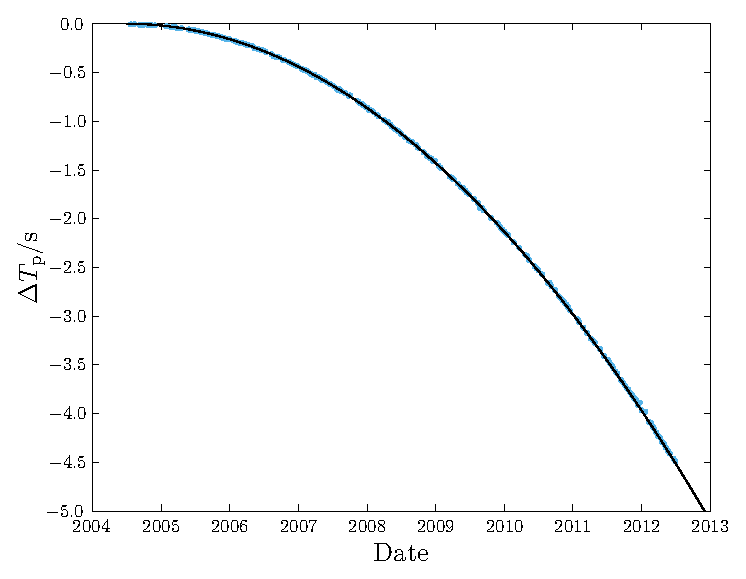
\includegraphics[width=0.7\textwidth]{./images/Fig_Pulsar}
    \caption{Evolution of the orbital parameters of the double pulsar system as quantified by the cumulative shift in periapse time since the beginning of observation $\Delta T\sub{p}$ \citep[cf.][]{Weisberg2010}. The points show the observations and the line indicates the GR prediction \citep{Kramer2008}. The error bars are smaller than the plotted point size. Without GW emission $\Delta T\sub{p} = 0$. Data courtesy of Michael Kramer.}   
    \label{fig:pulsar} 
\end{figure}
The observations are in excellent agreement with the expected GW inspiral. Thus, GWs have been indirectly detected.
There are a number of experiments designed to directly observe GWs \citep{Riles2012}. Modern detectors attempt to measure the minute changes in distance induced by a passing GW (\citealt[section 9.5]{Thorne1987}; \citealt[section 18.9]{Hobson2006}). The amplitude of a GW is characterised by a strain: the fractional change in length resulting from the perturbation from the background spacetime.

The Laser Interferometer Gravitational-wave Observatory (LIGO; \citealt{Abramovici1992}) and the European Gravitational Observatory's Virgo detector \citep{Acernese2008a}, which work in collaboration, are currently being upgraded to their advanced configurations (aLIGO and aVirgo) and are expected to make the first detection shortly after recommencing operation around 2015 \citep{Harry2010,Accadia2011}.\footnote{An optimistic hope is to celebrate the centenary of Einstein's 1916 prediction of GWs \citep[document 32]{Einstein1997} with the first direct detection.} These are ground-based interferometers that detect passing GWs by measuring the induced difference in the length of their two arms \citep{Pitkin2011}. They are sensitive to frequencies in the range $\sim10$--$10^4\units{Hz}$, with peak sensitivity at about $100\units{Hz}$. The LIGO and Virgo detectors are supported by GEO 600, a smaller interferometric experiment that incorporates prototype technologies \citep{Willke2002,Willke2006}. LIGO has two sites, one in Hanford, Washington and one in Livingston, Louisiana. The Hanford observatory has two detectors; the current design has one operate over half the arm-length of the other. There is an agreement to move one of the upgraded detector systems to a location in India \citep{Unnikrishnan2013}. The LIGO-India detector, operated by the Indian Initiative in Gravitational Observations (IndIGO), provides a longer baseline between detectors, giving improved sky location and sky coverage \citep{Schutz2011}.

A further ground-based interferometer is under construction in Japan. The Kamioka Gravitational Wave Detector (KAGRA), formerly the Large-scale Cryogenic Gravitational Wave Telescope (LCGT; \citealt{Kuroda1999,Kuroda2010}) will operate underground in the Kamioka mine. It lags several years behind the other detectors, aiming to start observations in 2017--2018, but will employ more sophisticated noise-reduction techniques such as cryogenic cooling \citep{Somiya2012}.

Ground-based GW astronomy may eventually be continued by the construction of the Einstein Telescope, an ambitious proposal to construct an underground detector with $10\units{km}$ arms \citep{Punturo2010,Hild2011,Sathyaprakash2012}. Its location would provide shielding from seismic noise, allowing it to observe frequencies $10$--$10^4\units{Hz}$. There is no definite time-line for this concept.

There is another contender for the first direct detection of GWs: PTAs \citep{McWilliams2012,Sesana2012a}. These infer the presence of a GW from periodic delays in the arrival times of the highly regular millisecond pulses from pulsars. In effect, the pulsars are used to create a detector with galactic-scale arms \citep{Hellings1983}. They are sensitive to frequencies of $\sim10^{-9}$--$10^{-7}\units{Hz}$. An international collaboration of European, North American and Australian radio telescopes is already in possession of the necessary instruments to detect GWs \citep{Hobbs2010}.\footnote{The International Pulsar Timing Array (IPTA) consortium consists of the European Pulsar Timing Array (EPTA), the North American Nanohertz Observatory for Gravitational Waves (NANOGrav) and the Parkes Pulsar Timing Array (PPTA) consortia.} The completion of the Square Kilometre Array (SKA; \citealt{Dewdney2009}) shall augment the search, greatly increasing sensitivity \citep{Kramer2004}.

Between the HF range of the ground-based detectors and the VLF range of PTAs lies a band that could be accessible to space-based interferometers. These are not limited by seismic noise and are free to have much longer arms than the ground-based detectors, making them sensitive to lower frequencies. The paragon detector design is the Laser Interferometer Space Antenna (LISA; \citealt{Bender1998, Danzmann2003}). This is a constellation of three satellites in a circular, heliocentric orbit forming a three-armed interferometer. Each arm is $5 \times 10^9\units{m}$, and the orbit trails $20^{\circ}$ behind the Earth. The detector is sensitive to a range of frequencies $\sim10^{-5}$--$1\units{Hz}$, having peak sensitivity around $10^{-3}$--$10^{-2}\units{Hz}$.

LISA developed as a joint NASA--ESA mission. In 2011 NASA withdrew for financial reasons leaving ESA to investigate reduced cost missions. The resulting descoped concept is the evolved Laser Interferometer Space Antenna (eLISA; \citealt{Jennrich2011, Amaro-Seoane2012a}).\footnote{This was submitted to the ESA for their L1 mission selection as the New Gravitational-wave Observatory (NGO).} This shares the same basic components as LISA but only has two arms and lags $9^{\circ}$ behind the Earth. The arms are $1 \times 10^9\units{m}$; this shifts the peak sensitivity to marginally higher frequencies, around $10^{-2}\units{Hz}$. Overall the noise curve is raised relative to LISA giving eLISA reduced sensitivity.

At the time of writing, there is no currently funded mission. However, LISA Pathfinder, a technology demonstration mission, is due for launch in 2015 \citep{Anza2005, Antonucci2012}. Hopefully, a full mission shall follow in the subsequent decade.\footnote{At the time of writing a science theme has been submitted to ESA for their L2/3 mission selection.}

In addition to the LISA family, there are other proposed space-borne detectors. The Japanese Deci-hertz Interferometer Gravitational Wave Observatory (DECIGO; \citealt{Kawamura2006,Kawamura2011}) consists of constellations of satellites similar to LISA, but with arms of $100\units{km}$ and an optical system similar to LIGO's. It fills the gap between the LISA family and the ground-based detectors, being most sensitive to frequencies $0.1$--$10\units{Hz}$. DECIGO could be scheduled for launch as early as 2027, pending the success of two pathfinder missions \citep{Ando2010}.

There have even been suggestions for successors to LISA \citep{Crowder2005}. The Advanced Laser Interferometer Antenna (ALIA; \citealt{Bender2013}) and the Big Bang Observer (BBO) are both popular concepts. Compared to the LISA family, they have shorter arms, making them sensitive to higher frequencies, and better sensitivities. They may be more comparable to DECIGO \citep{Yagi2011a}. These designs are highly speculative.

\subsubsection{Gravitational wave sources}\label{sec:GW-sources}

GWs can be emitted by a variety of systems. To produce detectable signals the source must consist of extremely massive objects moving at a significant fraction of the speed of light. The quintessential source is a binary of two COs. These inspiral as a result of GW emission and eventually merge. There is a wide range of binary systems; examples include:
\begin{itemize}
\item Compact binaries (CBs) made up of two closely-orbiting stellar-mass COs, most commonly white dwarfs (WDs). These are the end result of the stellar evolution of a binary star system \citep{Postnov2006}. Wider CBs in the Galaxy are a source for LISA-like detectors. These are so common that some may form an unresolvable foreground for LISA \citep{Nelemans2009}; others would be guaranteed sources allowing us to verify the functionality of the detector \citep{Stroeer2006}. At the end of the inspiral, the system merges in a CB coalescence (CBC). This produces a target signal for ground-based detectors \citep{Abadie2010a} as well as a potential EM counterpart \citep[e.g.,][]{Webbink1984,Iben1984Jr,Metzger2010,Rezzolla2011,Nakar2011}. Observations of CBs will help us to understand stellar evolution, in particular common envelope evolution \citep{Ivanova2013}.

\item MBH binaries consisting of two BHs with masses $\gtrsim 10^5 M_\odot$ \citep{Sesana2013b}; BHs at the upper end of the mass spectrum ($\gtrsim10^8$--$10^9 M_\odot$) are sometimes referred to as supermassive black holes (SMBHs). MBHs are found in the centre of galaxies \citep{Lynden-Bell1969,Ferrarese2005}. When galaxies merge, their MBHs also spiral together \citep{Volonteri2003,Schnittman2013}. The inspiral, merger and subsequent ring-down of the new MBH are all promising sources of GWs \citep{Flanagan1998}. Mergers are potentially the loudest GW signals. The combination of many inspirals should result in a stochastic background observable with PTAs \citep{Sesana2008}.

\item Extreme-mass-ratio (EMR) systems of a stellar-mass CO orbiting an MBH. They evolve slowly as a consequence of their large mass-ratio \citep{Glampedakis2005,Barack2009}. EMR systems with highly eccentric orbits produce a burst of GWs as they pass through periapsis; these are EMRBs and are in the frequency range of a LISA-like detector \citep{Rubbo2006}. EMR systems with near-circular orbits, which are expected in the last few years of inspiral prior to plunge, emit continuously within LISA's frequency band. These signals are extreme-mass-ratio inspirals (EMRIs; \citealt{Amaro-Seoane2007}). EMRIs can be observed over many orbits, allowing exquisitely high signal-to-noise ratios (SNRs) to accumulate. This makes them excellent probes of the background geometry permitting both precision measurements of the system parameters and tests of GR \citep[e.g.,][]{Babak2010}.
\end{itemize}
In addition to binaries, there are other potential sources of GWs. Supernovae are highly energetic, asymmetric explosions when a giant star ejects its outer envelope as its core collapses to an NS or BH; these generate HF bursts of GWs \citep{Dimmelmeier2002,Kotake2006}. Rotating NSs are a source of continuous HF GWs if they possess some degree of axial asymmetry \citep{Abbott2007,Prix2009}. More speculatively, early Universe processes, such as inflation \citep{Grishchuk2005} or a first-order phase transition \citep{Binetruy2012}, could have created GWs. Cosmic strings have also been hypothesised as a potential source \citep{Damour2005,Binetruy2012}. These relic GWs have been predicted across a range of frequencies and their discovery would be an exciting probe of the Universe before the emission of the CMB. Measuring the properties of GWs can tell us both about their source and the nature of gravity.

\section{Astrophysical compact objects}\label{sec:COs}

To probe regions of strong gravity we need COs. These are provided in nature through the remnants of stellar evolution \citep[section 1.1]{Shapiro1983}. Depending upon its mass, a star may end its life as a WD, NS or BH. More massive BHs can be found in the centres of galaxies; these have grown through accretion and mergers from a seed population that is poorly understood \citep{Volonteri2010}.

\subsection{White dwarfs and neutron stars}

The least massive stars ($\sim0.6$--$8M_\odot$) end their lives as WDs \citep{Poelarends2008}. These are made of electron-degenerate matter that form from the stellar cores once their outer envelopes are lost \citep{Althaus2010}. WDs' faint luminosity comes from thermal emission. Over billions of years they cool and dim, eventually fading from view \citep[section 4.2]{Shapiro1983}.

WDs have a maximum mass set by electron degeneracy pressure. This is known as the Chandrasekhar limit and is around $1.4 M_\odot$ (\citealt[section 3.4]{Shapiro1983}; \citealt{Nomoto1987,Timmes1996}). %\footnote{It is possible for WDs to collapse at lower masses during electron-capture supernovae.}
Above this the WD will collapse under its weight until neutron degeneracy pressure takes over to balance gravity. We then have a remnant NS or, if the mass is too large for neutron degeneracy to support, a BH \citep{Woosley2002,Langer2012}.

NSs form from stars of initial masses $\gtrsim 8$--$12 M_\odot$ \citep{Woosley2002,Poelarends2008,Langer2012}. They are made of nuclear-density material. The behaviour of matter under these extreme conditions is not well understood, leading to a plethora of different equations of state \citep{Lattimer2012}. Probing the strong-field regions around NSs could not only provide a test of our understanding of gravitation, but also elucidate the properties of extremely dense matter \citep[e.g.,][]{Read2009,Ozel2009,Lackey2012}.

The maximum mass of an NS depends upon its equation of state \citep[section 9.3]{Shapiro1983}. Hence there is no definitive theoretical prediction.\footnote{The most famous upper mass is the Tolman--Oppenheimer--Volkoff limit \citep{Tolman1939,Oppenheimer1939}. This model is known to be inadequate as the calculated mass is too small.} The largest current estimate for an NS mass is $2.74 \pm 0.21 M_\odot$ \citep{Freire2008,Ozel2012}. Once the maximum NS mass is exceeded, the gravitational force becomes overwhelming and the material is crushed down to become a BH \citep[section 12.1]{Shapiro1983}. The initial stellar mass required for a star to end its life as a BH is uncertain, but is estimated to be $\gtrsim 25 M_\odot$ \citep{Woosley2002,Tauris2011}.

\subsection{Black holes}

BHs are fascinating objects: beautifully simple but with many complexities in their interactions. \citet{Michell1784} first theorised a BH. This is not the same as the object that we understand today, but a Newtonian analogue: a star so massive that its escape velocity exceeds the speed of light. A general relativistic BH was first described with the much celebrated Schwarzschild solution \citep{Schwarzschild1916}. Discovered shortly after Einstein's publication of his general theory, this was the first exact solution other than flat spacetime. It is the metric for the space surrounding a spherically symmetric distribution of matter. It also describes a non-rotating, uncharged BH. A BH is a region of spacetime where gravity is so intense that there exists an event horizon, from within which nothing can escape \citep[section 33.1]{Misner1973}. The nature of BHs was not fully comprehended until many years after Schwarzschild published his metric; astrophysicists had to first realise the existence of WDs and NSs before they could accept the concept of completely collapsed objects \citep{Israel1987}.

Following on from Schwarzschild's discovery came the solution of \citet{Reissner1916} and \citet{Nordstrom1918} for an electrically charged BH. There was then a long hiatus before \citet{Kerr1963} discovered the metric for a rotating BH. The set of BH solutions was completed by the discovery of the Kerr--Newman metric for charged, rotating BHs \citep{Newman1965}. According to the no-hair theorem, any BH should be described completely by just its mass $M_\bullet$, spin and electric charge \citep{Israel1967, Israel1968, Carter1971, Hawking1972, Robinson1975}. We expect the charge of an astrophysical BH to be negligible, hence we only need two parameters to describe the BHs of nature \citep[sections 36, 51]{Chandrasekhar1992}.

Astrophysical BHs are grouped by their mass. We shall discuss three partitions: stellar-mass BHs, intermediate-mass BHs (IMBHs) and MBHs. MBHs are of major interest in this work and we pay them special attention.

The spin parameter $a$ is related to the BH's angular momentum $J$ by
\begin{equation}
J = M_\bullet ac;
\end{equation}
it is often convenient to use the dimensionless spin
\begin{equation}
a_\ast = \dfrac{cJ}{GM_\bullet^2}.
\end{equation}
The spin has a range of possible values $0 \leq |a_\ast| \leq 1$ \cite[section 66]{Chandrasekhar1992}. A spin $a_\ast = 0$ corresponds to a non-rotating BH. In general BHs shall have some angular momentum, and so we are mostly concerned with the Kerr solution.

\subsubsection{Stellar-mass black holes}

Stellar-mass BHs are an endpoint of stellar evolution, the product of the collapse of giant stars too massive to form NSs \citep{Postnov2006}. These have masses of order of a few solar masses. Observations show a distribution of $\sim5$--$10M_\odot$ \citep{Ozel2010,Farr2010} and stellar evolution models predict remnant masses of $\sim3$--$10M_\odot$ at solar metallicity, with higher masses being possible for lower metallicities \citep{Woosley2002}. BHs can also form following an NS merger \citep{Rezzolla2011,Faber2012}. Much of our understanding of these BHs comes from observations of X-ray binaries where the presence of a BH is illuminated by the accretion of matter from a companion \citep{Shakura1973,Remillard2006}.

\subsubsection{Intermediate mass black holes}

IMBHs bridge the gap between the other two classes. They are less well studied than the others, and lack concrete observational confirmation \citep{Miller2009a}, but have been proposed as a tentative explanation for some ultraluminous X-ray sources \citep{Feng2011}. They potentially represent an intermediate stage in the evolution of MBHs \citep{Graham2013}.

\subsubsection{Massive black holes}

MBHs have masses $\sim10^5$--$10^{10} M_\odot$. Many, if not all, galactic nuclei have harboured an MBH during their evolution \citep{Lynden-Bell1971, Soltan1982, Rees1984}. Observations have shown that there exist well-defined correlations between the MBHs' masses and the properties of their host galaxies, such as: bulge mass \citep{Kormendy1995,Haring2004,Graham2012a}; luminosity \citep{Magorrian1998,Marconi2003,Graham2013}; velocity dispersion \citep{Ferrarese2000,Gebhardt2000,Tremaine2002,Graham2011}; light concentration \citep{Graham2001}, S{\'e}rsic index \citep{Graham2007a,Savorgnan2013}, and, for spiral galaxies, pitch angle \citep{Seigar2008,Berrier2013}. These suggest coeval evolution of the MBH and galaxy \citep{Peng2007, Jahnke2011}, possibly with feedback mechanisms coupling the two \citep{Haiman2004, Volonteri2009}. The MBH and the surrounding spheroidal component share a common history, such that the growth of one can inform us about the growth of the other.
%m Kormandy1995; Magorrian1998; Haring2004; (breaking) Graham2012a; (breaking) Scott2013
%L Magorrian1998; Marconi2003; Graham2007; Gultekin2009; Graham2013; 
%sigma Ferrarese2000; Gebhardt2000; Tremaine2002; Gultekin2009; Graham2011
%C Graham2001
%n Graham2001; Graham2007a; Savorgnan2013
%P Seigar2008; Berrier2013

The best opportunity to study MBHs comes from the compact object in the Galactic centre (GC), which is coincident with the radio source Sagittarius A* (Sgr A*). Through careful monitoring of stars orbiting the GC, this has been identified as an MBH of mass $M_\bullet \simeq 4 \times 10^6 M_\odot$ at a distance of only $R_0 \simeq 8\units{kpc}$ \citep{Gillessen2009, Meyer2012}.

The masses of other MBHs have been determined using a selection of techniques. Aside from being inferred from the correlations enumerated above, they can be measured directly using stellar or gas dynamical observations \citep[e.g.,][]{Macchetto1997,vanderMarel1998,Gebhardt2003} or maser measurements of the velocity of a circumnuclear disc \citep[e.g.,][]{Miyoshi1995}. After measuring the masses of MBHs we are left with the question of their spins.

The spin of an MBH is determined by several competing processes. An MBH accumulates mass and angular momentum through accretion \citep{Volonteri2010,King2013}. Accretion from a massive gaseous disc shall tend to spin up the MBH, potentially leading to high spin values \citep{Volonteri2005}, while a series of randomly orientated accretion events leads to a low spin value: we expect an average value $|a_\ast| \sim 0.1$--$0.3$ \citep{King2006, King2008}. The MBH also grows through mergers \citep{Yu2002, Malbon2007}. Minor mergers with smaller BHs can decrease the spin \citep{Hughes2003, Gammie2004}, while a series of major mergers, between similar mass MBHs, would lead to a likely spin of $|a_\ast| \sim 0.7$ \citep{Gonzalez2007, Berti2007, Berti2008}. Measuring the spin of MBHs shall help us understand the relative importance of these processes, and perhaps shall give a glimpse into their host galaxies' pasts.

Elliptical and spiral galaxies are believed to host MBHs of differing spins because of their different evolutions: we expect MBHs in elliptical galaxies to have on average higher spins than MBHs in spiral galaxies, where random, small accretion episodes are thought to have played a more important role \citep{Volonteri2007, Sikora2007}.

It has been suggested that the spin of the Galaxy's MBH could be inferred from careful observation of the orbits of stars within a few milliparsecs of the GC \citep{Merritt2010}, although this is complicated because of perturbations due to other stars, or from observations of quasi-periodic oscillations in the luminosity of flares believed to originate from material orbiting close to the innermost stable orbits \citep{Genzel2003a, Belanger2006, Trippe2007, Hamaus2009, Kato2010}, though there are difficulties in interpreting these results \citep{Psaltis2008a}.

%This latter method, combined with a disc-seismology model, has produced a value of the dimensionless spin of $a_\ast = 0.44 \pm 0.08$. To obtain this result \citet{Kato2010} have combined their observations of Sgr A* with observations of galactic X-ray sources containing solar mass BHs, to find a best-fit unique spin parameter for all BHs. However, it is not clear that all BHs should share the same value of the spin parameter; especially considering that the BHs considered here differ in mass by six orders of magnitude, with none in the intermediate range. Even if BH spin is determined by a universal process, we still expect some distribution of spin parameters \citep{King2008, Berti2008}. Thus we cannot precisely determine the spin of the Galactic Centre's MBH from an average including other BHs.

A further possibility is to use VLBI to resolve features of the size of the order of the event horizon \citep{Doeleman2008,Fish2010}. The Galactic MBH, as a consequence of its mass and proximity, is the prime candidate, subtending about $50\units{\upmu as}$ on the sky \citep{Broderick2009a,Johannsen2012a}. With this capability, it would be possible to directly image accretion flows down to the horizon and also observe the MBH's shadow. This is the dark region surrounding the BH from which no light can reach the observer; it is bounded by the innermost photon orbit \citep[section 63]{Chandrasekhar1992}. The position of the horizon and the exact shape of the shadow are determined by the metric. By measuring them it may be possible to measure the spin and inclination of the BH \citep{Hioki2009a}, assuming it is Kerr, check whether it is an over-extreme Kerr BH \citep{Bambi2009}, or even probe deviations from Kerr \citep{Johannsen2010a, Johannsen2010b}.%\footnote{Observing deviations from Kerr would disprove the no-hair theorem (possibly admitting naked singularities); suggest a compact object described by an alternative metric such as a Manko-Novikov solution \citep{Manko1992, Gair2008}; provide evidence for a non-GR theory of gravity, or some combination of these options.}
The shape of the shadow of a Kerr BH is shown in \figref{Shadow}.
\begin{figure}%[htb]
\vspace{0.5\baselineskip}
  \centering
   \subfigure[$a_\ast = -0.2$, $\theta\sub{obs} = \pi/2$]{\resizebox{0.3\textwidth}{!}{\import{./Images/}{Shadow_2-psfrag.tex}}} \quad
   \subfigure[$a_\ast = -0.2$, $\theta\sub{obs} = \pi/6$]{\resizebox{0.3\textwidth}{!}{\import{./Images/}{Shadow_2_6-psfrag.tex}}} \quad
   \subfigure[$a_\ast = 0.4$, $\theta\sub{obs} = \pi/2$]{\resizebox{0.3\textwidth}{!}{\import{./Images/}{Shadow_4-psfrag.tex}}} \\
   \subfigure[$a_\ast = 0.4$, $\theta\sub{obs} = \pi/6$]{\resizebox{0.3\textwidth}{!}{\import{./Images/}{Shadow_4_6-psfrag.tex}}} \quad
   \subfigure[$a_\ast = 0.9$, $\theta\sub{obs} = \pi/2$]{\resizebox{0.3\textwidth}{!}{\import{./Images/}{Shadow_9-psfrag.tex}}} \quad
   \subfigure[$a_\ast = 0.9$, $\theta\sub{obs} = \pi/6$]{\resizebox{0.3\textwidth}{!}{\import{./Images/}{Shadow_9_6-psfrag.tex}}} \\
   \subfigure[$a_\ast = 0.998$, $\theta\sub{obs} = \pi/2$]{\resizebox{0.3\textwidth}{!}{\import{./Images/}{Shadow_998-psfrag.tex}}} \quad  
   \subfigure[$a_\ast = 0.998$, $\theta\sub{obs} = \pi/6$]{\resizebox{0.3\textwidth}{!}{\import{./Images/}{Shadow_998_6-psfrag.tex}}}
    \caption{Apparent shape of a Kerr BH shadow viewed from infinity, $\alpha$ and $\beta$ are the position coordinates projected onto the sky, and $\theta\sub{obs}$ is the polar coordinate of the observer \citep[section 63]{Chandrasekhar1992}. The shadow is circular when viewed along the spin axis ($\theta\sub{obs} = 0, \pi$).} 
    \label{fig:Shadow}
\end{figure}
The shadow remains near circular for spin values $|a_\ast| \lesssim 0.9$ regardless of inclination even though the Kerr spacetime is highly non-spherically symmetric \citep{Johannsen2010b}. Weak constraints already exist from VLBI observations \citep{Broderick2009a,Broderick2011}; these determine that the spin is likely not high: $|a_\ast| = 0$--$0.64$ at $68\%$ confidence and $|a_\ast| = 0$--$0.86$ at $95\%$ confidence. Determining the spin to high precision is difficult. 

The spins of MBHs in active galactic nuclei have been inferred using X-ray observations of $\mathrm{Fe}$ $\mathrm{K}$ emission lines \citep{Miller2007, McClintock2011}. So far this has been done for a handful of other galaxies' MBHs, as shown in \tabref{X-ray}.
\begin{table}\footnotesize
\centering
\begin{tabular}{l D{,}{.}{3.11} l }
\toprule
\multicolumn{1}{c}{AGN} & \multicolumn{1}{c}{$a_\ast$} & \multicolumn{1}{c}{Study} \\ \midrule 
1H 0323$+$342 & >0,37 & \citet{Walton2013} \\ % 90%
1H 0419$-$577 & >0,89 & \citet{Walton2013} \\ % 90%
1H 0707$-$495 & \geq 0,976 & \citet{Zoghbi2010} \\ % 90%
3C 120 & 0,994^{+0.002}_{-0.003} & \citet{Lohfink2013} \\
3C 382	& <0,81 & \citet{Walton2013} \\ % 90%
%Ark 120 & $<0.94$ & \citet{Patrick2011} \\ % 90%
Ark 120 & 0,74^{+0.19}_{-0.50}{^\dagger} & \citet{Nardini2011} \\ % 99% confidence
 & 0,64^{+0.19}_{-0.11} & \citet{Walton2013} \\ % 90%
Ark 564 & 0,96^{+0.01}_{-0.07} & \citet{Walton2013} \\ % 90%
Fairall 9 & 0,60 \pm 0.07{^\ast} & \citet{Schmoll2009} \\ % 68%
 & 0,44^{+0.04}_{-0.11} & \citet{Patrick2011} \\ % 90%
 & 0,39^{+0.48}_{-0.30} & \citet{Emmanoulopoulos2011} \\ % 90%
 & 0,67^{+0.10}_{-0.11} & \citet{Patrick2011a} \\ % 90%
 & 0,52^{+0.19}_{-0.15} & \citet{Lohfink2012} \\ % 90%
 & 0,82^{+0.09}_{-0.19} & \citet{Walton2013} \\ % 90% 
IRAS 00521$-$7054 & 0,97^{+0.03}_{-0.13} & \citet{Tan2012} \\ % 90%
IRAS 13224$-$3809 & 0,988 \pm 0.001{^\ast} & \citet{Fabian2013} \\ % 68%
%MGC$-$02-14-009 & $<0.88$ & \citet{Patrick2011} \\ % 90%
MCG$-$6-30-15 & 0,989^{+0.009}_{-0.002} & \citet{Brenneman2006} \\ % 90%
 & 0,86^{+0.01}_{-0.02} & \citet{delaCallePerez2010} \\ % 90%
 & 0,49^{+0.20}_{-0.12} & \citet{Patrick2011a} \\ % 90%
Mrk 79 & 0,7 \pm 0.1 & \citet{Gallo2011} \\ % 90%
Mrk 110 & 0,96^{+0.03}_{-0.07} & \citet{Walton2013} \\ % 90%
Mrk 335 & 0,70^{+0.12}_{-0.01} & \citet{Patrick2011} \\ % 90%
 & 0,83^{+0.09}_{-0.13} & \citet{Walton2013} \\ % 90%
Mrk 359 & 0,66^{+0.30}_{-0.54} & \citet{Walton2013} \\ % 90%
Mrk 509 & 0,78^{+0.03}_{-0.04} & \citet{delaCallePerez2010} \\ % 90%
 & 0,36^{+0.20}_{-0.37} & \citet{Walton2013} \\ % 90%
Mrk 841 & >0,52 & \citet{Walton2013} \\ % 90%
Mrk 1018 & 0,58^{+0.36}_{-0.54} & \citet{Walton2013} \\ % 90%
NGC 1365 & \geq 0,84 & \citet{Risaliti2013} \\ % 90%
NGC 3783 & \geq 0,88{^\dagger} & \citet{Brenneman2011} \\ % 99%
 & < 0,32 & \citet{Patrick2011a} \\ % 90%
NGC 4051 & < 0,94 & \citet{Patrick2011a} \\ % 90%
NGC 7469 & 0,69^{+0.09}_{-0.09} & \citet{Patrick2011} \\ % 90%
 & 0,64^{+0.13}_{-0.20} & \citet{Walton2013} \\ % 90%
%RBS 1125 & $\geq 0.60$ & \citet{Minniutti2010} \\ % Determined from soft excess smoothness which requires a high degree of relativistic blurring, rather than the relativistic iron line shape.
PDS 456 & >0,96 & \citet{Walton2013} \\ % 90%
PKS 0558--504 & >0,95 & \citet{Walton2013} \\ % 90%
RBS 1124 & >0,97 & \citet{Walton2013} \\ % 90%
SWIFT J0501.9$-$3239 & >0,99 & \citet{Walton2013} \\ % 90%
SWIFT J2127.4+5654 & 0,6 \pm 0.2 & \citet{Miniutti2009} \\ % 90%
 & 0,70^{+0.10}_{-0.14} & \citet{Patrick2011} \\ % 90%
Ton S180 & 0,92^{+0.03}_{-0.11} & \citet{Walton2013} \\ % 90%
UGC 6728 & >0,71 & \citet{Walton2013} \\ % 90%
 \bottomrule
\end{tabular}
\caption{Measurements of MBH spin from iron emission lines. Confidence levels are $90\%$ except where indicated otherwise: an asterisk ($^\ast$) is used for $68\%$ and an obelisk ($^\dagger$) is used for $99\%$. The scatter in results indicates the complexities of modelling the accretion disc.}\label{tab:X-ray}
\vspace{-3pt}
\end{table}
Estimates for the spin cover a range of values up to the maximal value for an extremal Kerr black hole. Typical values are in the intermediate range of $a_\ast \sim 0.7$ and above with an uncertainty of about $10\%$ on each measurement. There may be an observational bias toward high spin values \citep{Brenneman2011}.

%While we can use the spin of other BHs as a prior, to inform us of what we should expect to measure for the spin of the Galaxy's MBH, it is desirable to have an independent observation, a direct measurement.

%An exciting means of inferring information about the MBH is through GWs emitted when compact objects (COs), such as stellar mass BHs, neutron stars (NSs), white dwarfs (WDs) or low mass main sequence (MS) stars, pass close by \citep{Sathyaprakash2009}. A space-borne detector, such as the Laser Interferometer Space Antenna (LISA) or the evolved Laser Interferometer Space Antenna (eLISA), is designed to be able to detect GWs in the frequency range of interest for these encounters \citep{Bender1998, Danzmann2003, Jennrich2011, Amaro-Seoane2012a}. The identification of waves requires a set of accurate waveform templates covering parameter space. Much work has already been done on the waveforms generated when companion objects inspiral towards an MBH \citep{Glampedakis2005, Barack2009}; as they orbit, the GWs carry away energy and angular momentum, causing the orbit to shrink until eventually the object plunges into the MBH. These systems are typically formed following two-body encounters so that the initial orbits are highly eccentric; a burst of radiation is emitted during each periapse passage. These are extreme mass-ratio bursts (EMRBs; \citealt{Rubbo2006}). Assuming that the companion is not scattered from its orbit, and does not plunge straight into the MBH, its orbit evolves, becoming more circular, and it shall begin to continuously emit significant gravitational radiation in the LISA/eLISA frequency range. The resulting signals are extreme mass-ratio inspirals (EMRIs; \citealt{Amaro-Seoane2007}).

\section{Modified gravity}\label{sec:alternative}

GR is a remarkably successful theory. It satisfies every weak-field theory experiment we have currently devised \citep{Will2006}. However, there may yet be modifications to be revealed in strong-fields. Whilst we have no definite evidence that GR is not the correct classical theory of gravitation, there remain unanswered questions about gravity: What are the true natures of dark matter and dark energy? How should we formulate a quantizable theory of gravity? What drove inflation in the early Universe \citep{Guth1981,Lyth1999}? Therefore, there is motivation for exploration of alternative theories.

Studying modified gravity can be done in two ways: either studying specific alternative theories of gravity to discover what differences manifest, or looking for more general deviations from GR and then using these to constrain possible alternative theories.

\subsection{Alternative theories of gravity}

There is a plethora of modified gravity theories \citep{Clifton2012}. Perhaps the most infamous is the hypothesis of modified Newtonian dynamics (MOND; \citealt{Famaey2012}). Suggested by \citet{Milgrom1983a,Milgrom1983b,Milgrom1983c} to match observations of galaxies, Newtonian dynamics is modified at low accelerations such that
\begin{equation}
\mu\left(\dfrac{a}{a_0}\right)\boldsymbol{a} = \boldsymbol{g}
\end{equation}
where $\boldsymbol{g}$ is the Newtonian gravitational field strength, $\boldsymbol{a}$ is the acceleration, $a_0 \approx 10^{-10}\units{m\,s^{-2}}$ is the new acceleration scale and $\mu$ is an interpolation function with properties $\mu(x) \rightarrow 1$ for $x \gg 1$ and $\mu(x) \rightarrow x$ for $x \ll 1$. There is a variety of relativistic theories that can reproduce this behaviour, including Einstein--\ae{}ther theory and tensor--vector--scalar (TeVeS) theory \citep{Bekenstein2006}. The hypothesis works well for describing galactic-scale systems but is not as successful, compared with the standard cold dark matter paradigm, at larger scales, for example, describing the properties of galaxy clusters \citep{Aguirre2001,Angus2007}. It may be possible to constrain MOND theories in the low-acceleration regime by using LISA Pathfinder to measure the acceleration at the Earth--Sun saddle point \citep{Magueijo2011,Galianni2011}. Most alternative theories, however, reduce to the Newtonian limit in the weak field.

Alternative theories of gravity can be created by adding new fields or modifying the form of the gravitational action \citep{Gair2012a}.\footnote{Here ``or'' is inclusive. In some cases, a modification of the gravitational action can be recast as introducing a new field \citep[e.g.,][]{Wands1994,Jacobson2010}.} We shall describe a few to illustrate the range of possibilities.

Including a scalar field in addition to the metric tensor produces scalar--tensor gravity \citep{Wagoner1970,Nordtvedt1970Jr,Fujii2003}. The best known example is Brans--Dicke gravity; this has a scalar field replace the gravitational constant \citep{Brans1961,Dicke1962}. Deviations from GR can be quantified in terms of the Brans--Dicke coupling parameter $\omega\sub{BD}$, as $\omega\sub{BD} \rightarrow \infty$ observable differences become smaller, while in a natural theory we might expect $\omega\sub{BD} \sim \order{1}$. Measurements of light deflection from the Cassini--Huygens mission \citep{Bertotti2003} constrain Brans--Dicke to be close to GR with the bound $\omega\sub{BD} > 4 \times 10^4$ \citep{Will2006}.

Vector--tensor gravity introduces a vector field \citep{Will1972Jr,Nordtvedt1972Jr}. This is typically time-like and in Einstein--\ae{}ther theory is constrained to have unit norm \citep{Jacobson2001,Jacobson2008}. These theories have a preferred reference frame specified by the vector field. Preferred frame effects can be constrained by careful observational measurements \citep[chapter 8]{Will1993}.

%Tensor--tensor or bimetric theories have a second metric.

Scalar--vector--tensor gravities have the gravitational field couple to both vector and scalar fields. It is the natural extension to scalar--tensor and vector--tensor gravity. TeVeS includes a metric tensor, a unit vector field, one dynamical scalar field and one non-dynamical scalar field \citep{Bekenstein2004,Skordis2009}. It has three parameters (one setting a length-scale, the others dimensionless) and a free function that can be tuned to either recover MOND or Newtonian behaviour in the weak-field limit, and become arbitrarily close to GR. Bi-scalar--tensor--vector gravity generalises TeVeS by introducing a second dynamical scalar field in place of the non-dynamical field \citep{Sanders2005}. A separate theory is scalar--tensor--vector gravity which contains a vector field and three scalar fields, one of which replaces the Newtonian constant $G$, in addition to a metric \citep{Moffat2006}. This includes an additional repulsive Yukawa force in the weak-field limit. The added freedom of including extra fields allows fitting of a wide range of phenomena.

In $f(R)$-gravity the Einstein--Hilbert action is generalised by exchanging the Ricci scalar $R$ for an arbitrary function $f(R)$ \citep{Buchdahl1970, Sotiriou2010, DeFelice2010}. The action may be further generalised by using an action including other contractions of the Riemann tensor, such that it becomes $f(R, R_{\mu\nu}R^{\mu\nu}, R_{\mu\nu\rho\sigma}R^{\mu\nu\rho\sigma})$ \citep{Madsen1989, Farhoudi2006, Nojiri2011}. These higher-order gravities, so-called because the action contains derivatives higher than second-order (as in GR), have a rich variety of phenomenology. The flexibility in defining the form of the arbitrary function allows them to be fitted to a range of observations.

Motivated by gauge theories, Chern--Simons gravity includes a term in the action proportional to the Pontryagin density ${^\ast R} R = (1/2)\epsilon^{\nu\rho\sigma\tau}{R^\lambda}_{\mu\sigma\tau}{R^\mu}_{\lambda\nu\rho}$, where $\epsilon^{\nu\rho\sigma\tau}$ is the Levi-Civita alternating tensor, coupled to a (pseudo-)scalar field \citep{Jackiw2003, Smith2008, Alexander2009a}. This introduces gravitational parity violation and, consequently, this theory includes birefringent GWs, altered precession rates, and the modification of vacuum solutions that are axisymmetric but not spherically symmetric such as Kerr. GW observations could place tight constraints on any Chern--Simons correction \citep{Canizares2012}.

Ho\v{r}ava--Lifshitz gravity \citep{Horava2009, Sotiriou2009c, Blas2010a} sacrifices spacetime covariance in favour of being renormalizable. A preferred foliation of space and time along the lines of the Arnowitt--Deser--Misner formalism is adopted \citep{Arnowitt1962a}, with Lorentz invariance being emergent at large distances. This removes many of the problems regarding time traditionally associated with trying to quantize GR. However, there are outstanding problems in producing a viable theory consistent with observations \citep{Sotiriou2010a}.

\subsection{Deviations from general relativity}

Since there is a plethora of alternative theories, it is challenging to expound the observable consequences of all possibilities. Furthermore, it is possible that the true theory of gravitation is something yet to be conceived. It is therefore useful not only to look for the signatures of particular theories, but also to find generic tests that can be used to detect deviations from GR. If these deviations are not observed, we can be more confident in GR and place tighter constraints on viable alternatives, whilst if a deviation is discovered we can select suitable alternatives.

The parameterized PN (PPN) formalism provides a simple means of characterising gravity in the weak-field limit \citep[chapter 4]{Will1993}. The PPN framework describes deviations from Newtonian gravity. There are ten parameters: $\gamma$ which quantifies the space-curvature produced by a mass; $\beta$ which quantifies the non-linearity in the superposition law; $\xi$ which measures preferred-location effects; $\alpha_1$--$\alpha_3$ which quantify any preferred-frame effects, and $\zeta_1$--$\zeta_4$ (with $\alpha_3$) which measure non-conservation of momentum. These can differ in GR and alternative theories. Current PPN limits have been placed using a variety of tests, such as those discussed in \secref{exist-tests} \citep{Will2006}. The soon-to-be-launched Gaia mission, which shall provide high-precision astrometry measurements, shall give improved measurements of $\gamma$ and $\beta$ through careful monitoring of light-bending and the motion of asteroids \citep{Mignard2010, Hobbs2010a, Hestroffer2010}. Whilst PN parameters are useful in the weak-field, we wish to find strong-field equivalents.

The ideal probe of strong-field gravity is gravitational radiation. GWs can be modified in alternative theories of gravity. One modification is the addition of other polarizations. There may be up to six polarizations in a general metric theory (\citealt{Eardley1973}; \citealt[section 10.2]{Will1993}): as well as the two standard tensor modes, $h_+$ and $h_\times$, there can be two scalar modes (longitudinal and transverse) and two vector modes (assuming a wave propagating in the $z$-direction, one mode oscillates in the $x$--$z$ plane and another in the $y$--$z$ plane). These other polarizations are observable with GW detectors \citep{Tinto2010,Alves2011,Blaut2012}; their discovery would be decisive evidence against GR.

Restricting ourselves to the standard two polarizations, modifications to the gravitational waveform can be described in terms of the parameterized post-Einsteinian (PPE) framework \citep{Yunes2009a}. This follows in the footsteps of the PPN formalism by providing a set of parameters that can be adjusted to fit different theories. Constraining these can place limits on deviations from GR or select viable alternative theories \citep{Cornish2011}. The post-Einsteinian parameters were developed to describe the quasi-circular inspiral, merger and ring-down of binary non-spinning BH-like objects. Although designed for measuring anomalies in GWs, it is possible to impose some bounds on the plausible range of post-Einsteinian parameters using observations of binary pulsars \citep{Yunes2010}.

Measuring the propagation speed of GWs is another test of relativistic gravity \citep[section 10.1]{Will1993}. Any deviation from $c$ would be evidence for an alternative theory. This can happen in theories with massive gravitons \citep{Babak2003,Goldhaber2010}. In this event, GWs also become dispersive. If there are additional polarization modes, these can travel at different speeds. The GW speed can be measured by comparing arrival times for EM counterparts \citep[e.g.,][]{Cooray2004,Kocsis2008} or by monitoring the phase evolution of an inspiral \citep{Will1998,Berti2011}.

In addition to scrutinizing the gravitational radiation itself, we can use it to study its source. The BHs of GR are Kerr solutions and so specified entirely by their mass and spin. The mass multipole $M_\ell$ ($M_0 \equiv M_\bullet$) and mass-current multipole moments $S_\ell$ ($S_1 \equiv J/c$) are determined from these according to \citep{Hansen1974}
\begin{equation}
M_\ell + iS_\ell = M_\bullet \left(ia\right)^\ell.
\end{equation}
Checking this consistency relation for higher multipoles is a method of testing whether a CO is a Kerr BH as expected \citep{Gair2012}. For example, in Chern--Simons gravity, the BH solution differs at the fourth multipole \citep{Sopuerta2009a}.  The structure of the spacetime exterior to an object is determined by these multipole moments \citep{Geroch1970}. EMRI observations can be used to build a detailed map of the spacetime of a massive CO. Information regarding the multipole moments is encoded within the frequency spectrum of the GWs \citep{Ryan1995,Ryan1997}.

Introducing higher-order multipole moments results in the creation of a bumpy BH. These have been studied to discover the observable consequences of deviations from Kerr. A variety of different bumpy metrics have been considered; these include stationary and axisymmetric deformations of Schwarzschild which are solutions of the Einstein equations \citep{Collins2004} and, similarly, deformations of Kerr \citep{Vigeland2010a}; a quasi-Kerr metric with an arbitrary mass quadrupole \citep{Glampedakis2006a,Barack2007}; the metric of \citet{Manko1992}, which is a solution of Einstein's equations with arbitrary higher-order mass multipole moments \citep{Gair2008}; perturbed Kerr metrics that are not required to satisfy the Einstein equations but do preserve an approximate or an exact Carter-like constant \citep{Vigeland2011,Gair2011,Johannsen2013b}, and an axisymmetric Kerr-like metric, where the perturbations are different powers of $M_\bullet/r$, which is required neither to be a solution of the Einstein equations nor have full integrability of its geodesic motion \citep{Johannsen2011}. All these metrics deviate from the standard Kerr solution by a small amount and reduce down to it as the perturbation goes to zero; if the perturbation is large enough it can be detected with EMRIs.

%%The majority of the work to date has focused on spacetimes that are solutions in GR, but which deviate from the Kerr solution. However, if GR was not the correct theory of gravity, this could also lead to detectable signatures in the observed gravitational waves. Certain alternative theories of gravity, including $f(R)$, do admit the Kerr metric as a solution, since it has vanishing Ricci tensor, $R_{\mu\nu} = 0$~\cite{Psaltis2008, Yunes2011}. However, the Kerr metric need not be the expected end state of gravitational collapse~\cite{Barausse2008}. If a Kerr BH existed in an alternative theory, the geodesics would be the same, but the energy flux carried by the GWs could still be different, and so differences would show up in the rate of inspiral; although in many cases these differences do not appear at leading order. In most cases, however, either the Kerr metric is not admitted as a solution, or it is not the correct metric to describe collapsed objects~\cite{Yunes2011}. Waveform differences then show up as a result of the differences in the instantaneously-geodesic orbits of the compact object involved in the EMRI. Since the leading-order energy-momentum tensor of the GWs often takes the same form as in GR~\cite{Stein2011}, this is the primary effect and means the problem of testing alternative theories through EMRI observations is equivalent to the spacetime mapping programme within GR described previously.

%There are also certain qualitative features that could be smoking-guns for a departure from the Kerr metric, such as ergodicity in the orbits~\citep{Gair2008}, persistent resonances~\citep{Lukes-Gerakopoulos2010} or a shift in the frequency of plunge~\citep{Kesden2005, Gair2008}.

%%As a consequence of the difficulties of solving for GW emission in alternative theories, work on testing alternative theories of gravity using LISA EMRIs has so far been restricted to a few cases. In Brans-Dicke gravity, in which the gravitational field is coupled to a scalar field, differences show up due to a modification to the inspiral rate that arises from dipole radiation of the scalar field~\cite{Berti2005}. Neutron star EMRIs are required since the dipole radiation depends on a sensitivity difference between the two objects, and the sensitivity is the same for all BHs. Lower mass central BHs provide the most powerful constraints, but a LISA observation of a neutron star EMRI into a $10^4 M_{\odot}$ BH could place constraints on the Brans-Dicke coupling parameter that are competitive with Solar System constraints~\cite{Berti2005}. In dynamical Chern-Simons modified gravity, the action is modified by a parity-violating correction, inspired by string theory~\cite{Alexander2008, Alexander2009a}. In this case, the BH solution differs from the Kerr solution at the fourth multipole, $l = 4$, but the energy-momentum tensor of gravitational radiation takes the same form as in GR~\cite{Sopuerta2009a}. LISA observations of EMRIs should place constraints on the Chern-Simons coupling parameter that are an order of magnitude better than will be possible from binary pulsar observations, although a full analysis accounting for parameter degeneracies has not yet been carried out~\cite{Sopuerta2009a}. 

\section{General relativistic binaries}\label{sec:two-body}

A two-body system is the simplest case where we can study gravitational interactions. Therefore, it is necessary to have a good theoretical understanding of binary dynamics. Binary systems are also of fundamental importance for GW astronomy, where they are the principal source of radiation. The general relativistic two-body problem is difficult to model because of the theory's non-linearity. However, without understanding the predictions of GR it is impossible either to infer accurately the properties of astronomical bodies or to look for deviations from GR. Progress in understanding the two-body problem has been made in recent years; despite being well-studied there still remain open questions. The tools used to study a two-body system depend upon the field strength and the relative masses of the objects.

In weak fields, results can be obtained using PN calculations \citep{Blanchet2006}. These employ series expansions in powers of  $(v/c)^2 \sim \varepsilon$, where $v$ is the orbital speed. Each subsequent power is a higher PN order. Use of a PN expansion ensures the correct Newtonian limit is recovered. The PN calculations are well suited to modelling the behaviour of wide binaries and are commonly used to generate the early part of a GW inspiral template. However, other complementary approaches are required to model strong-field dynamics where a finite-term PN expansion is no longer accurate.

In strong fields, bodies of comparable mass can be studied using numerical relativity (NR; \citealt{Centrella2010,Pfeiffer2012,Sperhake2013}). In NR, the Einstein equations are solved directly using a computer. The spacetime is discretized and the metric is calculated for successive time steps. Rapid advances in this field have been made following breakthroughs in 2005 \citep{Pretorius2005,Campanelli2006,Baker2006}. NR simulations allow us to understand equal mass BH--BH mergers. These can be either stellar-mass BH mergers that are targets for ground-based GW detectors or MBH mergers that are potential sources for a space-borne detector. NR simulations produce accurate gravitational waveforms from inspiral through merger and ring-down. Comparison with PN waveforms shows reasonable agreement until late in the inspiral when the PN approximation breaks down \citep[e.g.,][]{Baker2007,Buonanno2007}. Whilst NR results are accurate, they are computationally expensive and so cannot be used to generate waveforms for large numbers of orbits.

Systems of unequal masses, where the masses differ by a factor of $10$--$100$ \citep{Lousto2010,Lousto2011}, are more challenging to evolve numerically as they complete a larger number of orbits and it is necessary to resolve two different scales. Progress in this area continues, but so far, numerical simulations for EMR systems have been limited to radial infall \citep{East2012}. Gravitational waveforms can instead be calculated using perturbative approaches (\citealt{Teukolsky1973}; \citealt[chapter 9]{Chandrasekhar1992}).

In the case of EMR systems, efforts are concentrated on understanding the gravitational self-force \citep{Barack2009,Poisson2004}. In the test particle limit the smaller body follows an exact geodesic of the MBH's spacetime. Including the effects of the smaller body's finite mass, the background spacetime is perturbed. The back-reaction from this deformation alters the small body's orbital trajectory, and can be modelled as a self-force that moves the body from its geodesic \citep{Mino1997,Quinn1997,Gralla2008}. It is analogous the EM  radiation reaction force that results from the interaction of an accelerating charge with its own field (\citealt{Dirac1938}; \citealt[sections 16.1--16.3]{Jackson1999}). The self-force is commonly divided into two pieces, dissipative and conservative. The former is time antisymmetric and encapsulates the slow decay of the orbital energy and angular momentum, constants of the motion in the test particle limit, through radiation. The latter is time symmetric and shifts the orbital phases inducing precession. The ability to accurately model the influence of the self-force should allow us to create accurate waveform models, and work in this area continues \citep[e.g.,][]{Pound2012}.

\section{Overview}

Developments in our theoretical understanding of gravity are driven by astronomical observations. Astrophysical systems are dominated by gravitational interactions; our understanding of them can be enhanced by using gravitational probes. To date, gravity has only been studied in the weak-field regime. Exploring the strong-field regime, as found around COs such as BHs, shall deliver new insights. We could learn about the evolution of MBHs, and by implication their surrounding galaxies, or uncover modifications to GR. One promising means of delving into the strong-field is through GW astronomy. This is in its infancy; what it shall teach us is yet to be revealed, but there is scope for exciting discovery.

We shall study what we learn from strong-field tests and GWs. In \partref{astro} we use GWs, specifically EMRBs, to learn about MBHs. We study the properties of EMRB waveforms (\chapref{waveforms}) and how they can be used to infer the properties of the Galactic MBH (\chapref{param}). The Galaxy's MBH, being the closest MBH, is the ideal system to study, but we shall also consider the possibility of bursts from extragalactic sources (\chapref{extragal}). We shall build a model to predict the Galactic event rate (\chapref{events}), which requires detailed calculations pertaining to the properties of the surrounding stellar cluster (\chapref{relax}). Our final result shall be an estimate for the information EMRB measurements could provide about the Galactic MBH. In \partref{grav} we look in detail at gravity itself; without understanding its behaviour we cannot interpret GW observations for astronomical purposes. We first investigate the observable signatures of metric $f(R)$-gravity. We calculate how GWs are modified within the alternative theory (\chapref{f-R1}) and then compute constraints that a viable theory must satisfy (\chapref{f-R2}). Our main result is a strict bound limit which must be satisfied by the function $f(R)$. After this (\chapref{resonances}), we study the effects of transient resonances in EMRIs. These are not currently included in waveform models, but could have measurable effects. Since we could not accurately measure the properties of an MBH or potential deviations from GR without suitable waveform templates, we investigate the effect that resonances could have. Studying EMRIs necessitates precise understanding of the general relativistic two-body problem and the gravitational self-force. In the course of this thesis, we shall learn about both gravitation and astrophysics.
